% QUESTAO
Determine o valor do lado $a$ no triângulo abaixo utilizando a Lei dos Cossenos:
(Considere $\text{cos}\,60^\circ = \frac{1}{2}$ e a fórmula $a^2 = b^2 + c^2 - 2bc \cdot \text{cos}\,\alpha$)

\parbox{0.3\linewidth}{

% ALTERNATIVAS
$\sqrt{19}$
$\sqrt{25}$
$5$
$\sqrt{13}$
$7$

}\parbox{0.7\linewidth}{
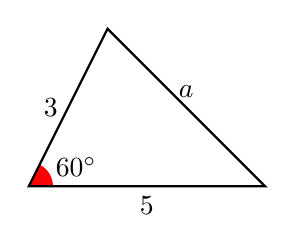
\begin{tikzpicture}[scale=1]
	\draw[red, fill] (0,0) -- (0.3,0) arc (0:60:0.3) -- cycle;
	\draw[thick] (0,0) -- (3,0) node[midway, below] {$5$} -- (1,2) node[midway, above] {$a$} -- cycle node[midway, left] {$3$};
	\node at (0.6,0.25) {$60^\circ$};
\end{tikzpicture}
}


